\chapter{Large Scale Fading}
\label{larg_fad}

Large scale fading \citep{large_scale_fade} \citep{large_scale_fade2} is a result of signal attenuation due to signal propagation over large objects caused by shadowing through surroundings like buildings,hills,trees, streets etc. and losing power. Shadowing is caused by blockage of large objects, where new waves get created as a result of the obstacle. %as there is not pure line of sight.
 And over the whole path it represents the average signal attenuation. An illustration of Shadowing can be seen on the following Figure:
 
\begin{figure}[H]
\centering
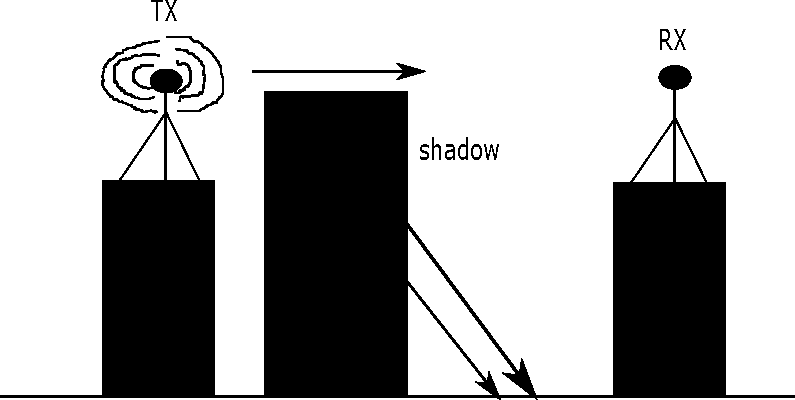
\includegraphics[width=0.6\textwidth]{shadow_ill.pdf}
\caption{Illustration of shadowing caused by an building in between the sender and the receiver}
\label{large_scale_shadow}
\end{figure}

 The path when working with large scale fading is of distances several hundred wavelengths or more. The wavelengths of course depends on the frequency. So when working with Bluetooth or Wi-Fi where the frequency is 2.4 [GHz]. 
%100 wavelengths is 12 [m]. 
Then given the equation for the wavelength:

\begin{equation}
\lambda = \frac{c}{f} = 12 [cm] 
\end{equation}

This gives us one wavelength, this means that for 100 wavelengths this shall be 12[m], which is then considered large scale fading. %In the free space case %with LOS conditions meaning no shadowing, and the receiver and transmitter can see each other with nothing blocking in between, 
%the attenuation of the signal due to distance follows the inverse square law given as:

%\begin{equation}
%\text{Average Signal Attenuation} = \frac{1}{d^{2}} 
%\label{inverse_square_law}
%\end{equation}  

%So the larger the distance from the transmitter to the receiver, the larger the signal attenuation will be. 
%\\
%\\
%In the case of effects caused by trees, buildings etc. The average signal attenuation cannot be characterized as the inverse square law given in \ref{inverse_square_law}, which only holds for free space. The effects of buildings, trees etc. are called shadows, which are waves that are caused by a building or something that is in the way, which creates new waves.
%when there is not pure LOS, meaning that a building or something is in the way, which creates new waves.
%\\
%\\
When taking shadowing into the equation a Lognormal Distribution is used to model the power variation, caused by the effects of shadowing \citep{large_scale_fade3}. The power level in dB is distributed as a Gaussian random variable. The power level in dB at a distance $d$ is given by the following equation:

\begin{equation}
P_{dB}(d) = \overline{P}_{dB}(d)+ \sigma_{dB}X = \overline{P}_{dB}(d_{0}) + 10n\log_{10}(\frac{d}{d_{0}})+ \sigma_{dB}X
\label{power_level}
\end{equation}     

Where $\sigma_{dB}$ is the standard deviation, and $X$ is a standard random variable. It shall be noted that knowledge of $\overline{P}_{dB}(d_{0})$ is required. $\overline{P}_{dB}(d_{0})$ is the path-loss at a distance $d_{0}$. 

A table for $\sigma_{dB}$ values can be seen on the following table:

\begin{figure}[H]
\centering
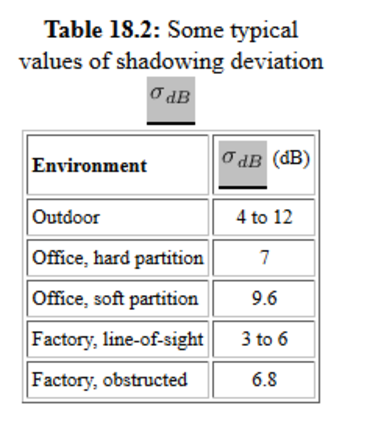
\includegraphics[width=0.3\textwidth]{standard_devi_largescale.pdf}
\caption{Table over the the standard deviation $\sigma_{dB}$ \citep{large_scale_fade3} }
\label{large_scale_shadow_stan_dev_val}
\end{figure}

Where $n$ is path loss exponent, where typical values of $n$ is given in the following table:

\begin{figure}[H]
\centering
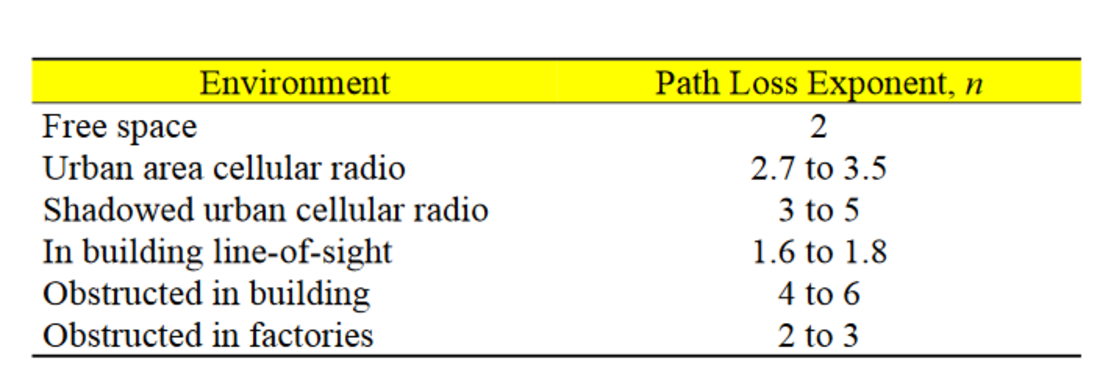
\includegraphics[width=0.6\textwidth]{pathloss_exp_n.pdf}
\caption{Table over the Path loss exponent $n$ \citep{large_scale_fade3} }
\label{large_scale_shadow_pathloss_expo_n}
\end{figure}

%, as the signal will be reflected of buildings.      %In the case of NLOS, which means that the receiver and the transmitter cannot see each other. 

%when working with long distances ()